% !Mode\dots ``TeX:UTF-8''
% !TEX root = ../bare_jrnl.tex


\section{The online observability of \BCNs}
\label{sec:online}

%In this section we propose the online observability to solve the problem mentioned in {\em Section \ref{sec:pre}}, and we will introduce its related information in detail. 
%
%In the rest of this section, firstly we introduce the inspiration for the online observability. Secondly we define derivation function. Thirdly we present the definition of $k$-step determinability. Finally, we give the formal definition of the online observability of \BCNs\ by derivation function and $k$-step determinability, and compare it with four existing observability.

%\subsection{Inspiration}


%As we mentioned in {\em Section \ref{sec:pre}}, we can determine the initial states of \BCNs\ by the third existing observability. \tl{(2)why but here?} But i
%{\color{red} (2)}In the third observability, the $\mathsf{s}(0)$ of a \BCN\ can be determined iff there exists an finite input sequence $\mathsf{I}$ that determine $\mathsf{s}(0)$.

%But we foud that we can derive the set of possible initial states $\mathsf{S}(0)$ by initial output $\mathsf{o}(0)$ we observe
%\[\mathsf{S}(0)=\{\mathsf{s}(0)\in \Delta_N|\ h( \mathsf{s}(0))=\mathsf{o}(0)\}.\]
%\tl{(3)i do not see logical connection here}
%Then if for every $\mathsf{S}^{i}(0)=\{\mathsf{s}(0)\in \Delta_N|\ h( \mathsf{s}(0))=\mathsf{o}^{i}(0)\}$, there is an input sequence $\mathsf{I}^{i}\in(\Delta_M)^k$ for some $k>0$, such that for any distinct states $\mathsf{s}^{x}(0)$, $\mathsf{s}^{y}(0) \in \mathsf{S}^{i}(0)$ implies $(HF)^k_{\mathsf{s}^{x}(0)}(\mathsf{I^i})\neq (HF)^k_{\mathsf{s}^{y}(0)}(\mathsf{I^i})$, we can determine the initial $\mathsf{s}(0)$ too. In this case, the requirements for a \BCN\ to determine its initial state would be easier to meet. \tl{(4)this because is connected to the previous sentence?}Because the corresponding input sequences $\mathsf{I}^{i}$ of different sets of possible initial states $\mathsf{S}^{i}(0)$ can be different. While in the third existing observability the $\mathsf{I}^{i}$ has to be identical.

%Furthermore, we can derive the set of possible states $\mathsf{S}(1)$ by the outputs $\mathsf{o}(0)$ and $\mathsf{o}(1)$ we observe and the input $\mathsf{i}(0)$ 
%\[\mathsf{S}(1)=\{\mathsf{s}(1)|\mathsf{s}(0)\in \mathsf{S}(0),\ \mathsf{s}(1)=f({\mathsf{i}(0)},{\mathsf{s}(0)}),\ h(\mathsf{s}(1))=\mathsf{o}(1)\}.\]

%And if for every $\mathsf{S}^{i}(1)$ we derived, 
%\begin{itemize}
%  \item  there is an input sequence $\mathsf{I}^{i}\in(\Delta_M)^k$ for some $k>0$, such that for any distinct states $\mathsf{s}^{x}(1)$, $\mathsf{s}^{y}(1) \in \mathsf{S}^{i}(1)$ implies $(HF)^k_{\mathsf{s}^{x}(1)}(\mathsf{I^i})\neq (HF)^k_{\mathsf{s}^{y}(1)}(\mathsf{I^i})$;
%  \item  and for every $\mathsf{s}^{x}(1)$ $\in \mathsf{S}^{i}(1)$ there exists only one corresponding $\mathsf{s}^{x}(0)$ $\in \mathsf{S}^{i}(0)$ such that $\mathsf{s}^{x}(1)=f({\mathsf{i}(0)},{\mathsf{s}^{x}(0)})$,
%\end{itemize} 
%then we can determine the initial state too. And in this case, the requirements for the \BCN\ to determine the initial state would be further easier to meet. Because the corresponding input sequences $\mathsf{I}^{i}$ of different sets of possible states $\mathsf{S}^{i}(1)$ can be different. 

%\tl{(5)this therefore is repeating what was said before?}
%Therefore, we have that if we utilize sets of possible states we derived more, it would be easier for a \BCN\ to meet the requirements to determine its initial state. According to this rule, we propose the online observability. 
%\tl{(6)does this mean that online observability is dependent on a particular rule?}

 Moreover, we find that to determine $\mathsf{s}(0)$ by taking the determining procedure once, we only need to complete the following procedure.

\begin{itemize}
\item At every time setp $t$, firstly, we observe the $\mathsf{o}(t)$ of \BCN, then based on $\mathsf{o}(t)=h(\mathsf{s}(t))$ we can infer the set of possible states $\mathsf{S}(t)$ by the $\mathsf{o}(t)$.
\item Secondly, with $\mathsf{S}(t)$ we can derive the set of possible inputs $\{\mathsf{i}_z(t),\ldots,\mathsf{i}_w(t)\}$, such that for every $\mathsf{i}^{i}(t)\in \{\mathsf{i}_z(t),\ldots,\mathsf{i}_w(t)\}$, for any two distinct $\mathsf{s}^{x}(t)$, $\mathsf{s}^{y}(t) \in \mathsf{S}(t)$, $f(\mathsf{s}^{x}(t), \mathsf{i}^{i}(t))\neq f(\mathsf{s}^{y}(t),\mathsf{i}^{i}(t))$. And then we choose $\mathsf{i}(t)$ from $\{\mathsf{i}_z(t),\ldots,\mathsf{i}_w(t)\}$.
\item Thirdly, based on $\mathsf{s}(t+1)= f({\mathsf{i}(t)},{\mathsf{s}(t)})$, $\mathsf{S}(t+1)$ is preliminarily derived, we need $\mathsf{o}(t+1)$ to further determine $\mathsf{S}(t+1)$. 
\end{itemize} 

$|\mathsf{S}(t+1)|\le|\mathsf{S}(t)|$, and we can determine $\mathsf{s}(t)$  when $|\mathsf{S}(t)|$ becomes $1$. Because for every $\mathsf{s}^{i}(t)\in $ $\mathsf{S}(t)$ there is exact one corresponding $\mathsf{s}^{i}(t-1)\in $ $\mathsf{S}(t-1)$, we can determine $\mathsf{s}(t-1)$, $\mathsf{s}(t-2)$, \ldots, $\mathsf{s}(0)$.
%And in this procedure, instead of finding the  $\mathsf{I}$ to determine $\mathsf{s}(0)$ before we take the determining procedure. We use the $\mathsf{S}(t)$ we derive at every time step $t$ to adaptively construct $\mathsf{I}$. 
Inspired by this procedure, we propose the online observability which states that a \BCN\ is observable if the previously mentioned procedure to determine $\mathsf{s}(0)$ can be completed {\bf definitely}.  We will formally define it in folllowing subsections, 
%\tl{(7)this implies that online is at least as powerful as offline, but why it is stronger?}
%Such that the requirements to determine the \BCNs' initial state would be easiest to meet. Thus, a \BCN\ satisfies the online observability iff its initial state $\mathsf{s}(0)$ can be determined for every $\mathsf{s}(0) \in \Delta_N$. 
its formal definition should define  
%After introducing the idea of the online observability, we briefly present how to determine the initial state of a \BCN. 
\begin{itemize}
\item the way to derive $\mathsf{S}(t)$ by $\mathsf{o}(t)$, $\mathsf{i}(t-1)$ and $\mathsf{S}(t-1)$ should be described, %So we define the derivation function to solve this problem.
\item  and the way to derive $\mathsf{i}(t)$ by $\mathsf{S}(t)$ to guarantee that $\mathsf{s}(0)$ can be determined. %Thus we define the $k$-step determinability for $\mathsf{S}(t)$ which means that we can determine $\mathsf{s}(t)$ by $\mathsf{S}(t)$ in $k$ time steps.
\end{itemize} 
%Therefore, we have the definition of the online observability that a \BCN\ is online observable if for every $\mathsf{S}^{i}(0)$ we derived, there exists a $k^i\ge 0$ such that the $\mathsf{S}^{i}(0)$ is $k^i$-step determinable.

%\tl{(8)this means that the "definition" is dependent on a particular way to define $S(t)$ and $i(t)$. In other words, if one gives a different way to define $S(t)$ and $i(t)$, you would have another definition of online observability. This suggests that the def of online observability is not robust.}


%-------------------------------------
\subsection{Derivation function}
%-------------------------------------
{\color{red} (9)} To describe how to derive $\mathsf{S}(t)$ by $\mathsf{o}(t)$, $\mathsf{i}(t-1)$, $\mathsf{S}(t-1)$ and the updating rules of \BCN, we define the derivation function $\Ded( \mathsf{S},  \mathsf{i},  \mathsf{o})$. %The definition of it is as follows.
\begin{definition}[$\Ded( \mathsf{S},  \mathsf{i},  \mathsf{o})$] 
%$2^{\Delta_N}$ be the power set of states; \tl{in a def, please do not introduce notations}
%$(\Delta_M\cup\varepsilon)$ be the set of inputs and $\varepsilon$ means empty input; 
%$(\Delta_Q\cup\varepsilon)$ be the set outputs and $\varepsilon$ means empty output.
\begin{equation*}
\begin{split}
&\Ded( \mathsf{S},  \mathsf{i},  \mathsf{o})=\{  \mathsf{s}'\in\Delta_N|\\
& \mathsf{s}'=\left\{
\begin{array}{rcl}
f( \mathsf{i}, \mathsf{s})      &      & {\mathsf{i}\neq \varepsilon}\\
\mathsf{s}       &      & {\mathsf{i}= \varepsilon}
\end{array} \right. ,  \mathsf{s} \in \mathsf{S}, \ h(\mathsf{s}')=\mathsf{o}\ if\ \mathsf{o}\neq \varepsilon\},
\end{split}
\end{equation*}
where $\mathsf{S}\in 2^{\Delta_N}$, $\mathsf{i} \in (\Delta_M\cup\varepsilon)$, $\mathsf{o} \in (\Delta_Q\cup\varepsilon)$, $\varepsilon$ presents empty input or output.
\tl{(9)I found hard to read this def.}
\end{definition}

 Then we have $\mathsf{S}(t)$ is defined as follows.{\color{red} (12)}
 \begin{definition}[$\mathsf{S}(t)$] In a \BCN, with the $\mathsf{i}(0)\mathsf{i}(1)\ldots\mathsf{i}(k-1)$ and $\mathsf{o}(0)\mathsf{o}(1)\ldots\mathsf{o}(k)$, we have for every $t\le k$, 
	\[\mathsf{S}(t)=\left\{
\begin{array}{rcl}
\Ded\left(\Delta_N,\varepsilon,\mathsf{o}(0)\right)      &      & {t=0}\\
\Ded\left(\mathsf{S}(t-1),\mathsf{i}(t-1),\mathsf{o}(t)\right)       &      & {t>0}
\end{array} \right. .\]

\end{definition}
\begin{example}
In the \BCN\ mentioned in {\em Example \ref{exa:2}}, if $\mathsf{o}(0)=\delta_4^0$, then \[\mathsf{S}(0)=\Ded\left(\Delta_N,\varepsilon,\delta_4^0\right)=\{\delta_{16}^0,\delta_{16}^1,\delta_{16}^2\}.\]
%If the possible states set $\mathsf{S}=\{\delta_{16}^0$, $\delta_{16}^1$, $\delta_{16}^2\}$ and we input $\delta_4^0$ observe $\delta_4^2$, then we can derive that the set of possible new states can be $\delta_{16}^{9}$ or  $\delta_{16}^{10}$.
 \label{exa:8}
 \end{example}   
 

 
 
\subsection{$K$-step determinability}
{\color{red} (10)} We propose the $\Ks(\mathsf{S}(t))$ for $\mathsf{S}(t)$ to depict we can determine the $\mathsf{s}(t)$ in $\Ks(\mathsf{S}(t)$ time steps for every $\mathsf{s}(t)\in \mathsf{S}(t)$. 
 \tl{(10)$k$-step determinability is a predicate, can you write in this form?}
\begin{definition}[$\Ks(\mathsf{S})$] 
For a non-empty $\mathsf{S}$
 \begin{itemize}
 \item   if $|\mathsf{S}|=1$ then $\Ks(\mathsf{S}$)=0;
 \item  if $|\mathsf{S}|>1$ and there is an input $\mathsf{i}^{x} \in \Delta_M$ such that
 \begin{itemize}
 \item  $|\Ded(\mathsf{S},\mathsf{i}^{x},\varepsilon)|=|\mathsf{S}|$,
 \item  $\Ks(\Ded(\mathsf{S},\mathsf{i}^{x},\mathsf{o}^{j}))< k$ for every non-empty $\Ded(\mathsf{S},\mathsf{i}^{x},\mathsf{o}^{j})$,
 \end{itemize} 
 and there is not any $\mathsf{i}^{y} \in \Delta_M$ such that
  \begin{itemize}
 \item  $|\Ded(\mathsf{S},\mathsf{i}^{y},\varepsilon)|=|\mathsf{S}|$,
 \item  $\Ks(\Ded(\mathsf{S},\mathsf{i}^{y},\mathsf{o}^{j}))< k-1$ for every non-empty $\Ded(\mathsf{S},\mathsf{i}^{y},\mathsf{o}^{j})$,
 \end{itemize} 
then $\Ks(\mathsf{S})=k$, where$k >0$;%, and we can input $\mathsf{i}^{i}$ to determine makes $\mathsf{S}$ $k$-step determinable.
 \item else $\Ks(\mathsf{S})=\infty$.
 \end{itemize}
\end{definition}

%Then, in order to better illustrate this definition, we give the following example.
\begin{example}\label{exa:9}
As mentioned in the {\em Example \ref{exa:8}}, $|\mathsf{S}(0)|=3$, as there exists $\delta_{4}^3$ such that 
 \begin{itemize}
 \item  $|\Ded\left(\mathsf{S}(0),\delta_{4}^3,\varepsilon\right)|=|\{\delta_{16}^0,\delta_{16}^{13},\delta_{16}^6\}|$,
 \item   and for each $\mathsf{o}^{j}\in \Delta_Q$
  \begin{itemize}
  \item   $\Ks(\Ded\left(\mathsf{S}(0),\delta_{4}^3,\delta_{4}^0\right))=\Ks(\{\delta_{16}^0\})=0$;
 \item  $\Ks(\Ded\left(\mathsf{S}(0),\delta_{4}^3,\delta_{4}^3\right))=\Ks(\{\delta_{16}^{13}\})=0$;
  \item  $\Ks(\Ded\left(\mathsf{S}(0),\delta_{4}^3,\delta_{4}^1\right))=\Ks(\{\delta_{16}^{6}\})=0$.
 \end{itemize}
 \end{itemize}
$\Ks(\mathsf{S}(0))=1$, $\mathsf{s}(0)$ can be determined in $1$ time step.
\end{example}  

We propose a lemma for $\Ks(\mathsf{S})$.

\begin{lemma}
For the non-empty $\mathsf{S}^{1}$ and $\mathsf{S}^{2}$, if $\mathsf{S}^{1}\subseteq\mathsf{S}^{2}$ and $\Ks(\mathsf{S}^{2})\ne\infty$, then $\Ks(\mathsf{S}^{1})\le\Ks(\mathsf{S}^{2})$.%and $\mathsf{S}^{1}\subseteq \mathsf{S}^{2}$, 
  \label{lemm:1}
\end{lemma}

%Because of the length of the article, we put all the proofs in the {\bf Appendix}. With the {\em Lemma \ref{lemm:1}}, it is easy to propose the {\em Lemma \ref{lemm:2}}
%\begin{lemma}
%For the non-empty $\mathsf{S}^{1}$ and $\mathsf{S}^{2}$, if $\mathsf{S}^{1}\subseteq\mathsf{S}^{2}$ and $\Ks(\mathsf{S}^{2})\ne\infty$ then $\Ks(\mathsf{S}^{1})\ne\infty$.
%For the sets of possible states $\mathsf{S}^{1}$ and $\mathsf{S}^{2}$, if there exists a $k^{i}\ge 0$ such that $\mathsf{S}^{2}$ is $k^{i}$-step determinable, and $\mathsf{S}^{1}\subseteq \mathsf{S}^{2}$, then there exists a $k^{j}\ge 0$ that $\mathsf{S}^{1}$ is $k^{j}$-step determinable.
%\label{lemm:2}
%\end{lemma}
All the proofs in the {\bf Appendix~A~Proof}. {\color{red} (11)}\tl{(11)give explicit reference.}

Then, we propose $\Ri(\mathsf{S}(t))$ to depict the set of inputs we can choose from to determine $\mathsf{s}(t)$.

\begin{definition}[$\Ri(\mathsf{S})$] 
\begin{equation*}
\begin{split}
&\Ri(\mathsf{S})=\{\mathsf{i}\in \Delta_M|\  |\Ded\left(\mathsf{S},\mathsf{i},\varepsilon\right)|=|\mathsf{S}|, \\
& \forall \mathsf{o} \in \Delta_Q, \Ded(\mathsf{S},\mathsf{i},\mathsf{o})\ne \emptyset \rightarrow \Ks(\Ded(\mathsf{S},\mathsf{i},\mathsf{o}))\ne \infty\}
\end{split}
\end{equation*}
\end{definition}
\begin{lemma}
For the non-empty $\mathsf{S}^{1}$ and $\mathsf{S}^{2}$, if $\mathsf{S}^{1}\subseteq\mathsf{S}^{2}$ and $\Ks(\mathsf{S}^{2})\ne\infty$, then $\Ri(\mathsf{S}^2)\subseteq\Ri(\mathsf{S}^1)$.
\label{lemm:2}
\end{lemma}

{\em Lemma \ref{lemm:1}} and {\em Lemma \ref{lemm:2}} can help us design the algorithm to determine the online observability of a \BCN.%, and we will represent the details in Section \ref{sec:deter}.
%==========================================================================================

\subsection{Online observability}
The online observability is formall defined as follows.

\begin{definition}[Online Observability of  BCNs]
\tl{(12)why $\epsilon$ is in the def? for which purpose?}
 A \BCN\ is online observable,
if for every non-empty $\Ded(\Delta_N,\varepsilon, \mathsf{o}^{j}(0))$, $\Ks(\Ded\left(\Delta_N,\varepsilon,\mathsf{o}^{j}(0)\right))\ne\infty$.
\end{definition}

%In order to better illustrate the definition of online observability, we give the following example.

\begin{example}
In the \BCN\ mentioned in {\em Example \ref{exa:2}}.  
 \begin{itemize}
 \item $\Ks(\Ded\left(\Delta_N,\varepsilon, \delta_{4}^0\right))=1\ne \infty$;
 \item $\Ks(\Ded\left(\Delta_N,\varepsilon, \delta_{4}^1\right))=1\ne \infty$;
 \item $\Ks(\Ded\left(\Delta_N,\varepsilon, \delta_{4}^2\right))=2\ne \infty$;
 \item $\Ks(\Ded\left(\Delta_N,\varepsilon, \delta_{4}^3\right))=2\ne \infty$.
 \end{itemize}
 
Therefore we have this \BCN\ is the online observable, we can determine the initial state of it by taking the determining procedure once. Comparing with {\em Example \ref{exa:6}} and {\em Example \ref{exa:7}}, the online observability can be used to determine the initial states of some \BCNs\ which can not be determined by existing observability. %Thus with the online observability we can research the \BCNs\ better.
\label{exa:10}
\end{example}  

\begin{lemma}
The online observability implies the  type-1 observability.
\label{lemm:3}
\end{lemma}

%With the existing first observability, we can distinguish every $\mathsf{s}^{i}(0)$ from other types of initial state, and we can also do this by the online obervability. Thus the online obervability implies the existing first observability. 

\begin{lemma}
The  type-3 observability implies the online observability.
\label{lemm:4}
\end{lemma}

From the {\em Lemma \ref{lemm:3}}, {\em Lemma \ref{lemm:4}}  and the implication relations between the existing four observability which mentioned in the {\em Section \ref{sec:pre}}, we have the relations among all five observability is shown in Fig.~\ref{fig:7}.
%In the existing third observability, we can determine the initial state $\mathsf{s}^{i}(0)$ of \BCN\ too. Thus the existing third observability implies the online obervability.

\begin{figure}[thpb]
      \centering
      \framebox{\parbox{3in}{\centerline{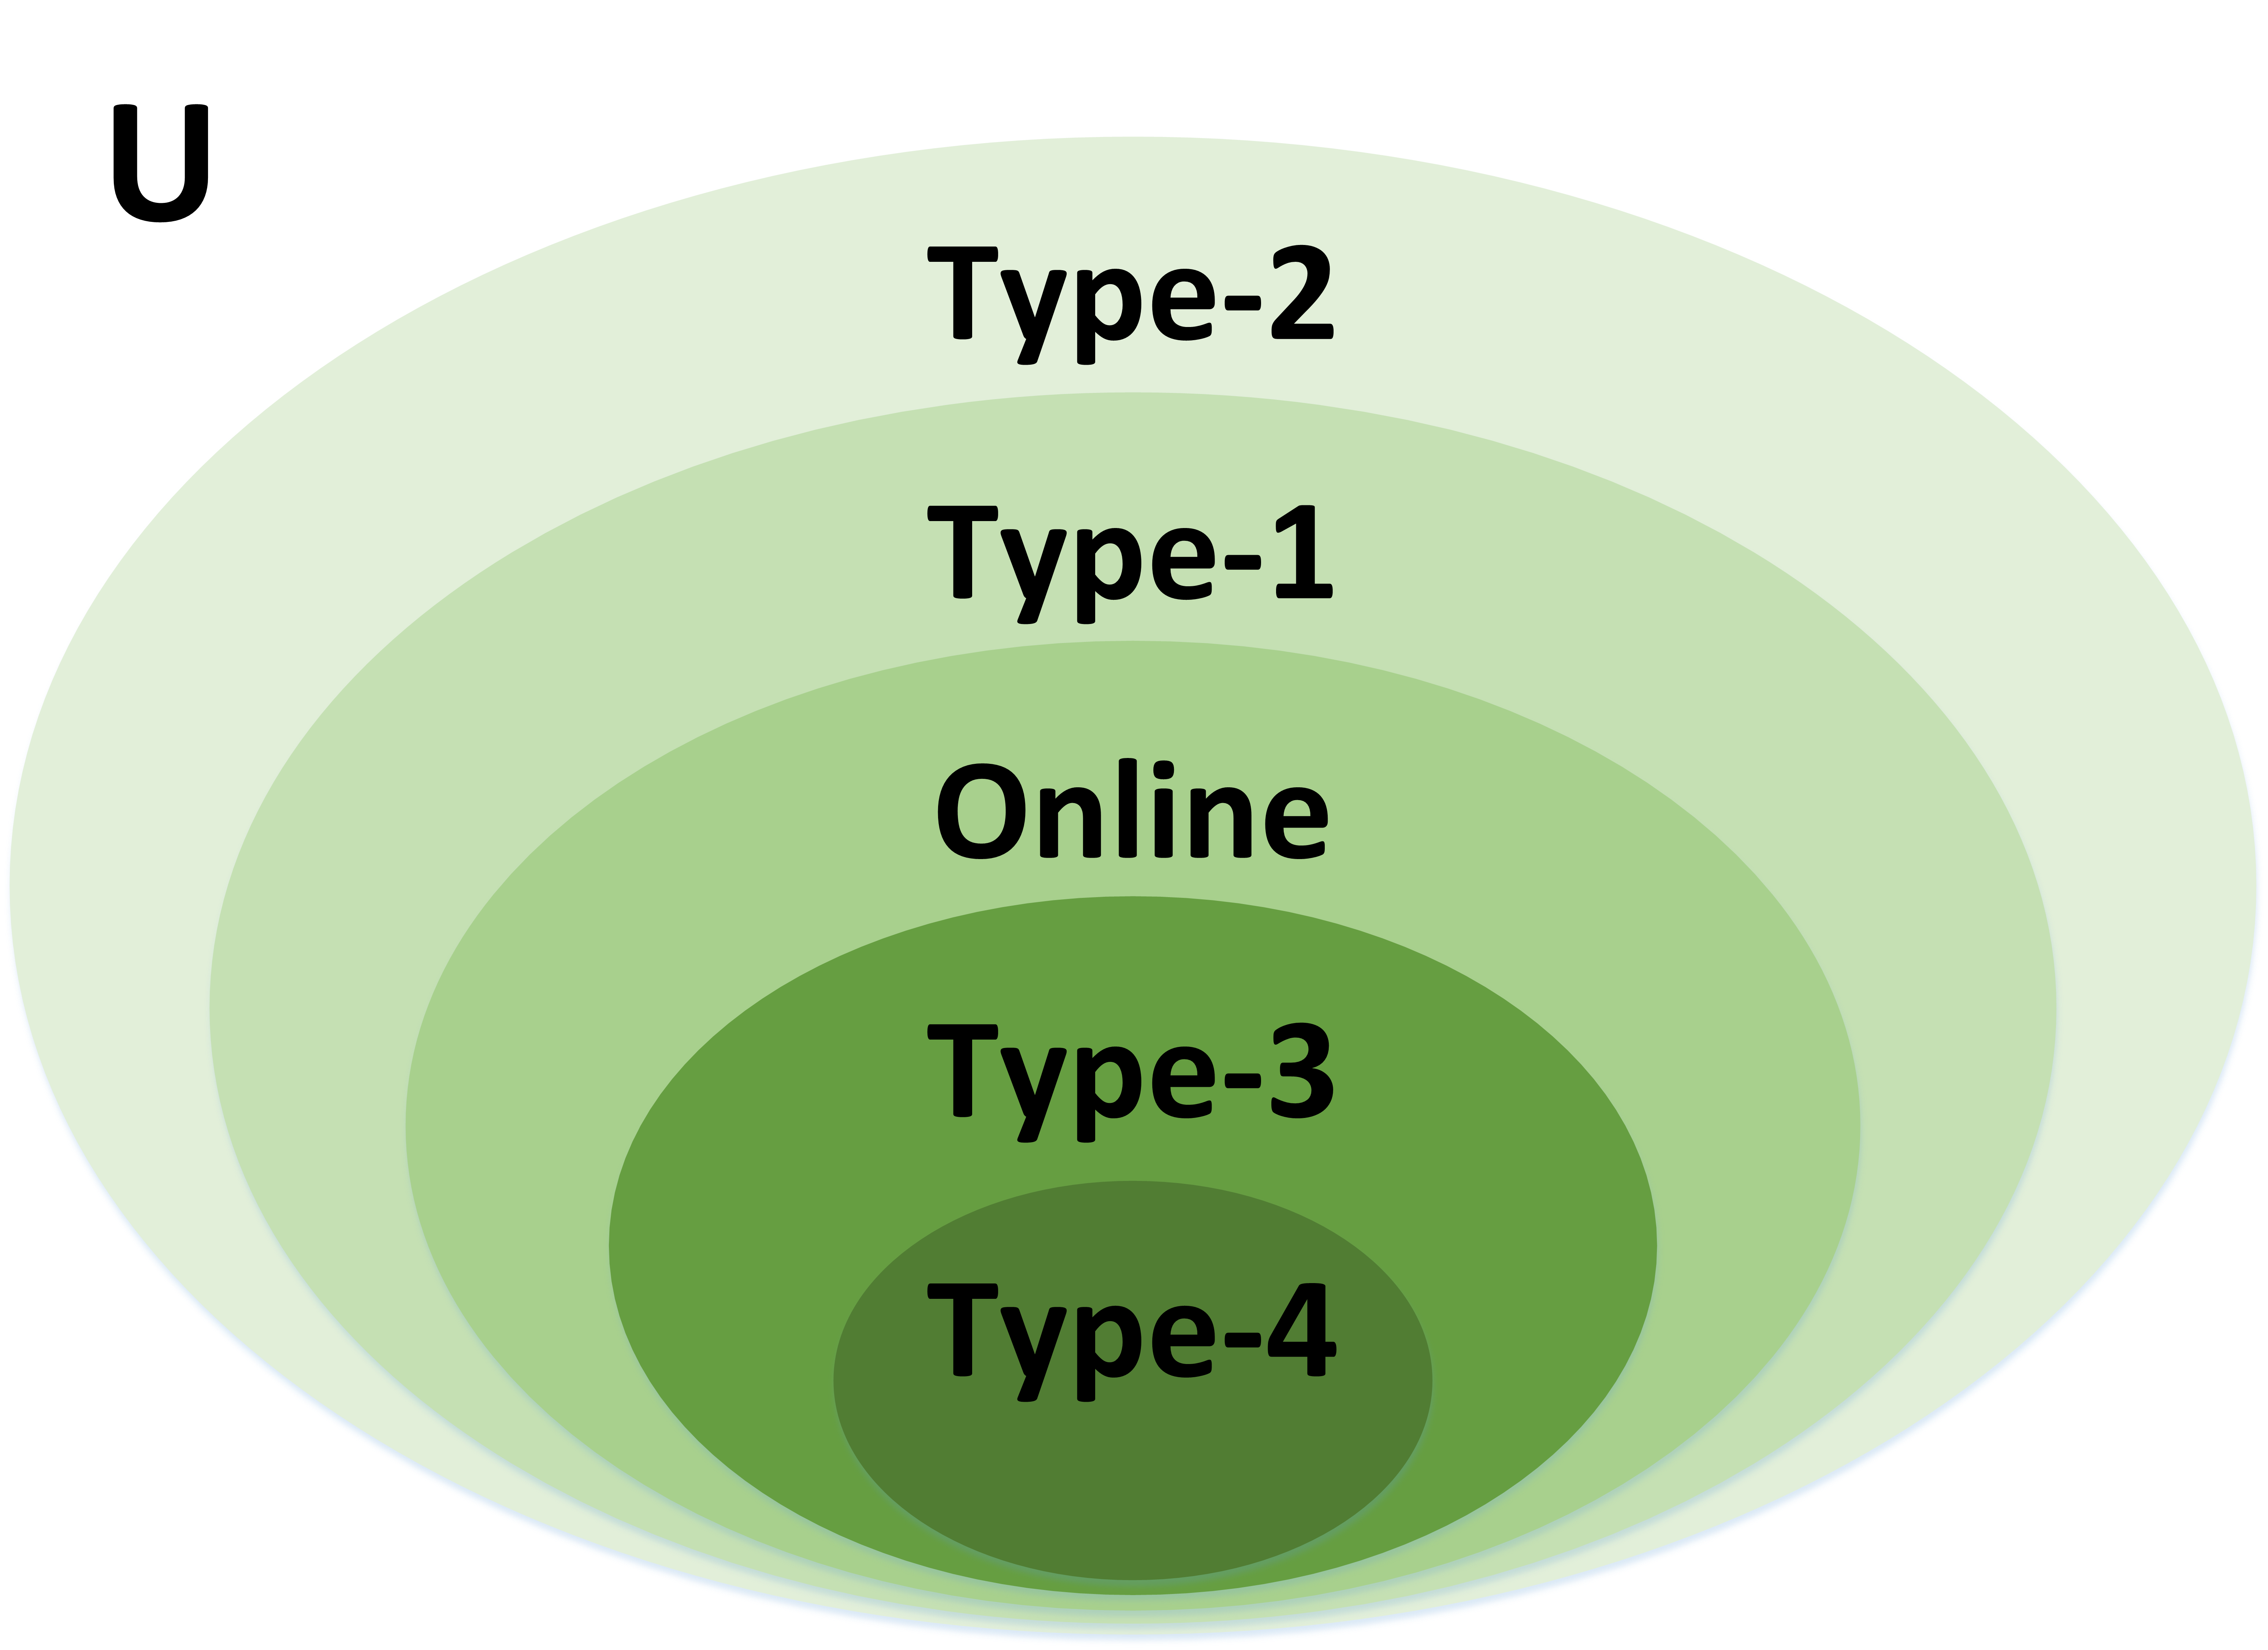
\includegraphics[scale=0.28]{figures/Fig11.png}} }} 
      \caption{The relationships graph between all five observability, where the area labelled with type of observability means the set of \BCNs\ which satisfy it and  ``U" means all of the \BCNs.}
      \label{fig:7}
   \end{figure}

\tl{(13)maybe you have done this, but I feel that one needs to highlight the advantages of this def. It is neither the strongest nor the weakest, why one should choose this?}

  {\color{red} (13)}In conclusion, the online observability addresses the necessary and sufficient condition of determining $\mathsf{s}(0)$ by taking the determining procedure once, because at every time step $t$, we observe $\mathsf{o}(t)$ of \BCN\ and choose $\mathsf{i}(t)$ based on the information we have collected so far. Such that the online observability enriches the control theory of \BCNs\ and determine the initial states of some \BCNs\ which can not be determined before. 